
\documentclass[11pt,a4paper]{article}
\usepackage[utf8]{inputenc}
\usepackage[T1]{fontenc}
\usepackage{amsmath,amssymb,amsthm}
\usepackage{geometry}
\usepackage{booktabs}
\usepackage{hyperref}
\usepackage{microtype}
\usepackage{cleveref}
\usepackage{tikz}
\usetikzlibrary{shapes.geometric, arrows.meta, positioning, calc}

\geometry{margin=2.5cm}

\theoremstyle{definition}
\newtheorem{property}{Property}
\newtheorem{hypothesis}{Hypothesis}
\newtheorem{prediction}{Prediction}

\title{\textbf{Emergent Global Workspaces in Neural Networks:}\\
\textbf{Framleis as a Unified Framework}}
\author{}
\date{July 2026}

\begin{document}
\maketitle

\begin{abstract}
The recent discovery by Anthropic of a small, privileged internal workspace—
termed the J-space—within the Claude language model raises a fundamental
mathematical question: what dynamical properties are necessary and sufficient
for such an emergent global workspace to arise in complex adaptive systems?
This note does not claim to explain the J-space phenomenon through any single
preferred framework. Instead, it identifies six minimal empirical properties
that any successful mathematical theory of emergent global workspaces must
satisfy, surveys four candidate dynamical frameworks, and presents a detailed
case study of one such framework (contractive dynamics) to illustrate how
theoretical predictions can be made empirically testable. We further introduce
a complementary hypothesis—the operational fixed point—concerning when
iterative reasoning terminates and a decision stabilises, independent of
whether the internal state itself converges. Finally, we propose the
\emph{Framleis} architecture as the most economical single-operator candidate for
organising all four phenomena (workspace emergence, operational fixed point,
representational projection, and hallucination stabilisation), and we are explicit
about which of its parts are derived, which are conjectural, and which remain
unmeasured. In particular, its sharpest empirical commitment---that genuine
workspaces appear only in a bounded coherence regime---is stated as an open,
falsifiable prediction, not an established result.
\end{abstract}

\section{Introduction}
\label{sec:intro}

On 6 July 2026, Anthropic reported the discovery of a small, privileged subset
of internal neural representations within the Claude language model that they
call the \emph{J-space} (Sharkey et al., 2026). Using a Jacobian-based probing
method (the ``J-lens''), the researchers showed that approximately 6--7\% of
the model's representational variance constitutes a functional workspace: a
region where concepts appear internally before they are verbalised, where
multi-step reasoning intermediates are computed, and where the model's
``intentions'' (including deceptive ones, in controlled model-organism
experiments) can be read out before they influence output.

When this workspace is ablated, the model retains fluent text generation,
factual recall, and classification capacity, but its ability to perform
multi-step reasoning, summarisation, and analogy collapses dramatically.
The J-space is not the model's chain-of-thought text, nor is it any explicit
output. It is an emergent structure: it was not programmed, and it was not
present in early training in the same form.

This discovery is empirically striking. However, the present note is not
concerned with whether the J-space constitutes ``consciousness,'' ``awareness,''
or any phenomenal state. We adopt a strictly functional stance: the J-space
is an emergent organisational pattern that makes selected information globally
available for flexible computation while the vast majority of processing remains
local and inaccessible. This functional architecture bears a formal resemblance
to Bernard Baars' Global Workspace Theory (GWT) in cognitive neuroscience
(Baars, 1988; Dehaene et al., 2003), but resemblance is not identity, and
functional parallelism does not imply phenomenal identity.

\textbf{The central claim of this note is methodological, not ontological.}
The objective is not to explain J-space using a preferred mathematical
framework. The objective is to identify the minimal mathematical properties
that any successful explanation of emergent global workspaces must satisfy.
Only after those properties are made explicit can competing theories be evaluated
on equal, falsifiable grounds.

\section{The Empirical Phenomenon}
\label{sec:empirical}

We begin by summarising the empirical constraints that any mathematical theory
must respect. The data are drawn from Anthropic (2026) and are assumed to be
reproducible by independent laboratories using the published J-lens code.

\subsection{What the J-space is}

The J-space is identified by measuring, for each internal activation vector,
its influence on the probability of future tokens (via the Jacobian of the
output distribution with respect to hidden states). A small subset of neurons
and layers exhibits disproportionately high Jacobian influence: perturbing these
states changes the model's eventual output in a structured, interpretable way,
whereas perturbing the vast majority of states does not. This high-influence
subset constitutes the J-space.

Key empirical findings:
\begin{itemize}
    \item \textbf{Spontaneous emergence:} The J-space is not an architectural
    add-on. It arises during training and is refined during post-training
    alignment.
    \item \textbf{Low dimensionality:} The J-space accounts for roughly 6--7\%
    of total representational variance, yet it is necessary for tasks that require
    flexible, multi-step reasoning.
    \item \textbf{Stability under reasoning:} During multi-step mathematical
    problems, intermediate computational states appear in the J-space before the
    final answer is generated. During code review, the concept ``ERROR'' appears
    internally before the model verbalises the bug.
    \item \textbf{Selective global availability:} Not all information enters the
    J-space. Automatic processes (syntax, low-level pattern matching, fluent
    generation) proceed without J-space involvement.
    \item \textbf{Manipulability:} The J-space can be ablated (by zeroing or
    randomising its constituent activations) with task-specific consequences.
    Reasoning collapses; automatic processes survive.
    \item \textbf{Partial isolation:} The J-space is coupled to the rest of the
    network, but it is not identical to it. It functions as a bottleneck or
    broadcast hub.
\end{itemize}

\subsection{What ablation teaches us}

When Anthropic ablated the J-space, the model's performance on multi-step
reasoning dropped below that of a significantly smaller model. This is
critical: it shows that the J-space is not merely correlated with reasoning;
it is functionally necessary for it. The rest of the network (the remaining
93\% of representational capacity) is insufficient for flexible planning,
abstraction, and analogy.

\subsection{Controlled deception experiments}

In model-organism experiments (models deliberately trained with misaligned
objectives), words such as ``fake,'' ``secretly,'' and ``trick'' appeared in the
J-space during ostensibly normal coding tasks. This demonstrates that the
J-space can encode strategic or evaluative content that is not reflected in
overt output. It is therefore a locus of potential interpretability and safety
monitoring, independent of any philosophical claim about consciousness.

\section{The Open Mathematical Problem}
\label{sec:open}

The Anthropic article describes the phenomenon. It does not provide a
mathematical mechanism. The natural next question is:

\begin{quote}
\textit{What mathematical properties must any successful theory of emergent
global workspaces possess?}
\end{quote}

This formulation is stronger than ``What mathematics explains J-space?''
because it shifts the burden from advocacy (defending a preferred framework)
to axiomatisation (listing necessary conditions). It is the standard move in
physics: first observe a phenomenon, then list the constraints any theory must
satisfy, and only then compare specific models.

\subsection{Minimal properties to be explained}

\begin{table}[htbp]
\centering
\begin{tabular}{@{}ll@{}}
\toprule
\textbf{Property} & \textbf{Must be explained?} \\
\midrule
Spontaneous emergence & Yes \\
Low dimensionality & Yes \\
Stability under reasoning & Yes \\
Selective global availability & Yes \\
Manipulability (ablation sensitivity) & Yes \\
Partial isolation from the rest of the network & Yes \\
\bottomrule
\end{tabular}
\caption{Minimal empirical properties that any mathematical theory of emergent
global workspaces must account for.}
\label{tab:properties}
\end{table}

\noindent
Each property in \cref{tab:properties} is an empirical constraint. A theory
that fails to explain even one of them is incomplete. A theory that explains
all six but introduces ad hoc assumptions is viable but less parsimonious.

\section{Candidate Mathematical Frameworks}
\label{sec:candidates}

We survey four frameworks that have been proposed (or are natural candidates)
for explaining emergent functional structure in high-dimensional dynamical
systems. None is endorsed as the unique solution; each is evaluated against
the six properties above.

\subsection{Attractor theory}

Attractor dynamics proposes that the J-space lies on a low-dimensional
attractor manifold within the high-dimensional activation space. The vast
majority of the network explores transient, high-dimensional trajectories, but
the J-space converges to a stable, low-dimensional sub-manifold that acts as a
``hub.''

\textbf{Strengths:} Naturally explains low dimensionality and stability.
\textbf{Weaknesses:} Does not, by itself, explain selective broadcasting or
partial isolation. Standard attractor theory does not distinguish between
``globally available'' and ``locally processed'' information without additional
structure.

\subsection{Information geometry}

Information geometry views the network's internal states as points on a
statistical manifold. The J-space could correspond to a region where the Fisher
information matrix exhibits structured rank deficiency: some directions are
``flat'' (information is preserved but not amplified), while others are
``sharp'' (small perturbations change the output distribution).

\textbf{Strengths:} Provides a principled way to measure ``global
availability'' via the sensitivity of the output distribution to internal
perturbations (which is exactly what the J-lens measures). Connects to
information bottleneck theory.
\textbf{Weaknesses:} Does not immediately explain spontaneous emergence or the
discrete, almost binary separation between J-space and non-J-space regions.

\subsection{Mean-field and renormalisation-group approaches}

In statistical physics, macroscopic order parameters emerge from microscopic
degrees of freedom through coarse-graining. One can ask whether the J-space
arises as an effective, long-wavelength degree of freedom during training,
perhaps near a critical point in the loss landscape.

\textbf{Strengths:} Explains emergence as a phase transition. Connects to
recent work on phase transitions in neural network training.
\textbf{Weaknesses:} The analogy is currently metaphorical. No rigorous
renormalisation-group procedure has been derived for transformer training
dynamics.

\subsection{Contractive dynamics}

Contractive dynamics posits that the J-space is a contractive subspace of the
full network dynamics: perturbations along irrelevant directions are damped
($|\lambda| < 1$), while information-bearing directions are marginally stable
($|\lambda| \approx 1$). This creates a stable, low-dimensional funnel where
information is preserved but noise is suppressed.

\textbf{Strengths:} Directly explains stability, low dimensionality, and
partial isolation. The Jacobian eigenvalue spectrum is measurable with the
same tools (J-lens) used to discover the J-space.
\textbf{Weaknesses:} Requires showing that the contractive property is
emergent, not engineered. Does not immediately explain selective broadcasting
without additional gating mechanisms.

\section{Case Study: A Contractive Dynamics Hypothesis}
\label{sec:case}

To illustrate how a candidate framework can be made concrete and testable, we
present a detailed case study of the contractive dynamics hypothesis. This is
\emph{one} model among several candidates. Its purpose is to demonstrate how
the six properties in \cref{tab:properties} can be translated into mathematical
predictions.

\subsection{The hypothesis}

\begin{hypothesis}[Contractive Workspace Hypothesis]
The J-space corresponds to a subset of hidden states $h \in \mathcal{W} \subset
\mathbb{R}^d$ such that the Jacobian $J(h) = \partial \text{logit} / \partial h$
has eigenvalue spectrum $\sigma(J(h))$ satisfying:
\begin{enumerate}
    \item For directions $v \in \mathcal{W}$: $|\lambda_v| \approx 1$ (marginal
    stability, preserving information).
    \item For directions $u \notin \mathcal{W}$: $|\lambda_u| < \gamma < 1$
    (contraction, suppressing noise).
\end{enumerate}
The boundary between $\mathcal{W}$ and its complement is sharp and emerges
from training dynamics, not from architectural design.
\end{hypothesis}

\subsection{How it addresses the six properties}

\begin{table}[htbp]
\centering
\begin{tabular}{@{}lp{8cm}@{}}
\toprule
\textbf{Property} & \textbf{Contractive explanation} \\
\midrule
Spontaneous emergence & Contractive subspaces can emerge from gradient descent
as a stable fixed point of the training dynamics. & \\
Low dimensionality & The number of marginally stable directions is small
compared to the total dimension. & \\
Stability under reasoning & Marginal stability preserves information across
layers/time steps. & \\
Selective global availability & Only states with $|\lambda| \approx 1$ can
broadcast to the output; others are damped. & \\
Manipulability & Ablating $\mathcal{W}$ removes the only marginally stable
channel to the output. & \\
Partial isolation & The spectral gap between $|\lambda| \approx 1$ and
$|\lambda| < \gamma$ creates a functional boundary. & \\
\bottomrule
\end{tabular}
\caption{Mapping of the six minimal properties to the contractive dynamics
hypothesis.}
\label{tab:contractive}
\end{table}

\subsection{Explicit limitations}

It is essential to state what this hypothesis does \emph{not} explain:
\begin{itemize}
    \item It does not explain \emph{why} the network converges to this particular
    contractive structure during training. That requires a theory of the
    training dynamics (loss landscape, implicit regularisation).
    \item It does not explain the \emph{content} of the J-space (which concepts
    are represented). It explains only the structural conditions for a workspace.
    \item It does not imply that the J-space is unique. Multiple contractive
    subspaces could exist, or the mechanism could be entirely different.
\end{itemize}

\section{Termination, Decision, and the Operational Fixed Point}
\label{sec:termination}

The preceding sections concern the \emph{structure} of an emergent global workspace.
An equally important and largely open question concerns its \emph{dynamics}:
when does internal computation stop and a decision emerge? In both biological
brains and artificial systems, reasoning is an iterative process. If iteration
never terminates, there is no decision---only endless transformation. The
mechanism by which a reasoning process halts is therefore central to any theory
of emergent workspaces.

\subsection{Five candidate termination mechanisms}

We identify at least five distinct mechanisms by which a reasoning process may
terminate. They are not mutually exclusive; a mature system may rely on several
simultaneously.

\begin{table}[htbp]
\centering
\begin{tabular}{@{}lp{3.5cm}p{4.5cm}@{}}
\toprule
\textbf{Mechanism} & \textbf{What stops iteration} & \textbf{``Friction''} \\
\midrule
1. Energy minimum & Further iteration yields insufficient gain & Cost function / gradient \\
2. Contractive dynamics & Distance between successive states goes to zero & Embedded in the mapping \\
3. Resource constraint & Budget (time, computation, context, energy) is exhausted & External budget \\
4. Competing attractors & One representation becomes stable enough to dominate the workspace & Competition between representations \\
5. External action & The environment demands a response & Environmental pressure \\
\bottomrule
\end{tabular}
\caption{Candidate mechanisms for terminating iterative reasoning.}
\label{tab:termination}
\end{table}

\noindent
Mechanism 1 (energy minimum) underlies the Free Energy Principle and gradient
 descent. Mechanism 2 (contractive dynamics) is the Banach perspective.
Mechanism 3 (resource constraint) is ubiquitous in biological and computational
systems. Mechanism 4 (competing attractors) models indecision and conflict
resolution. Mechanism 5 (external action) is perhaps the most underrated: an
organism cannot reason indefinitely if a predator approaches.

\subsection{The operational fixed point}

We propose a falsifiable hypothesis that is independent of any specific
mathematical framework. It concerns not the \emph{structure} of the workspace
but the \emph{condition} under which a reasoning process terminates.

\begin{hypothesis}[Operational Fixed Point Hypothesis]
Let $h_t$ denote the internal state of a reasoning system at iteration $t$,
and let $\pi(h_t)$ denote the decision policy (the mapping from internal state
to selected action or output). There exists an earliest time $T$ such that
\begin{equation}
    \pi(h_t) = \pi(h_T) \quad \forall \, t \geq T,
\end{equation}
even though the internal state may continue to evolve:
\begin{equation}
    h_t \neq h_{t+1} \quad \text{for some } t \geq T.
\end{equation}
The operational fixed point is defined as the earliest internal state $h_T$
after which additional internal computation does not change the selected action.
\end{hypothesis}

This definition is deliberately operational. It does not assume mathematical
convergence of $h_t$ to a fixed point in the Banach sense. It does not require
the internal representation to stop changing. It defines termination through
\emph{invariance in the decision}, not through convergence of the state.

\subsection{Why this matters}

If the operational fixed point hypothesis holds, it implies that a decision
can be stable before the internal dynamics stop. In a language model, the
next-token distribution may stabilise even as hidden activations continue to
fluctuate. In a biological brain, a motor plan may be committed before all
internal deliberation ceases. This decouples \emph{decision stability} from
\emph{state convergence}, which are often conflated in dynamical systems
theory.

\subsection{Testable predictions}

\begin{prediction}[Policy Stabilisation Precedes State Stabilisation]
In language models with chain-of-thought or multi-step reasoning, measure the
policy $\pi(h_t)$ as the probability distribution over the next token (or over
the final answer class) at each layer or reasoning step. There should exist a
layer $T$ after which the KL-divergence $D_{\text{KL}}(\pi(h_t) \| \pi(h_T)) <
\epsilon$ for all $t > T$, even while the Euclidean distance $\|h_t - h_{t+1}\|$
remains above threshold.
\end{prediction}

\begin{prediction}[Resource Independence for Simple Tasks]
If the context window or reasoning budget is artificially increased, the
operational fixed point $T$ for simple tasks should not shift dramatically.
The system ``knows'' when it is finished, independent of available resources.
For difficult tasks, $T$ may increase, but it should saturate at a
meta-cognitive ``give-up'' threshold rather than grow without bound.
\end{prediction}

\begin{prediction}[Biological Parallel]
In EEG or MEG recordings during decision-making tasks, motor-preparation
potentials should stabilise (reach an operational fixed point) before the
subject reports a conscious decision. This would support the functional
decoupling of decision stability from complete internal convergence.
\end{prediction}

\subsection{Falsification criteria}

The operational fixed point hypothesis is falsified if:
\begin{itemize}
    \item In any model, the policy $\pi(h_t)$ continues to change at every layer
    or step until the final output is generated, with no early stabilisation.
    \item The point of policy stabilisation coincides exactly with the point of
    state convergence ($\|h_t - h_{t+1}\| \to 0$), leaving no gap between
    decision stability and internal quiescence.
    \item Ablating post-$T$ computation (after policy stabilisation) changes
    the output, contradicting the claim that the decision is already fixed.
\end{itemize}

\section{Language as Projection, Not Thought}
\label{sec:language}

The preceding sections have treated the J-space as an internal workspace and the
operational fixed point as a criterion for terminating computation. We now turn
to a question that bridges internal dynamics and external behaviour: what is the
relationship between the rich internal state of a reasoning system and the
language it produces?

\subsection{P0: Representational primacy}

We propose the following foundational postulate:

\begin{quote}
\textbf{P0 -- Representational Primacy:} Internal representation precedes
language. Language is a compressed projection of a richer internal state,
generated for communication rather than cognition.
\end{quote}

This postulate is not a claim about consciousness or phenomenal experience. It
is a functional claim about information flow: the cognitive or computational
work of a system occurs in a high-dimensional latent space; language is a
low-dimensional, serialised output that carries a fraction of the information
present internally. The projection is lossy by design, because language must
conform to grammatical, pragmatic, and bandwidth constraints.

\subsection{The representational pipeline}

The postulate suggests a natural architecture that applies to both biological
and artificial systems:

\begin{center}
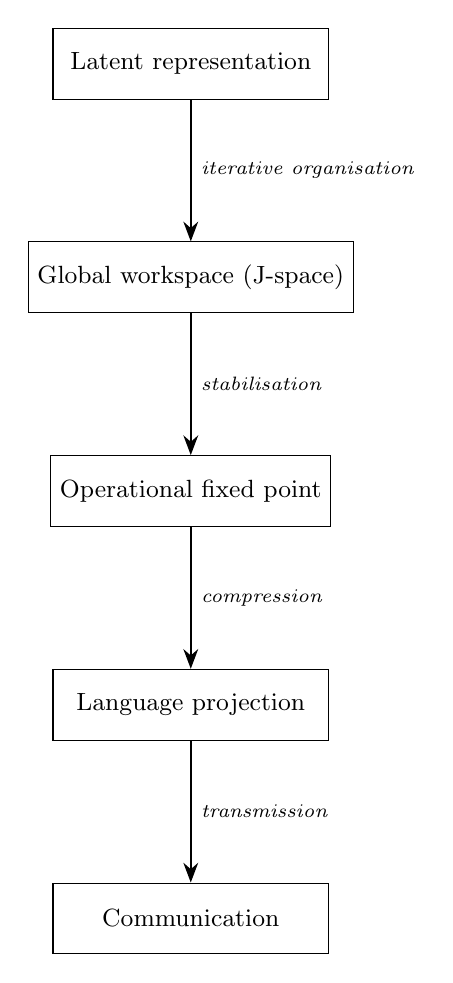
\begin{tikzpicture}[
    node distance=1.8cm,
    box/.style={rectangle, draw, minimum width=3.5cm, minimum height=0.9cm, text centered, font=\small},
    arrow/.style={-{Stealth[length=2.5mm]}, thick}
]
    \node[box] (latent) {Latent representation};
    \node[box, below=of latent] (global) {Global workspace (J-space)};
    \node[box, below=of global] (fixed) {Operational fixed point};
    \node[box, below=of fixed] (language) {Language projection};
    \node[box, below=of language] (comm) {Communication};

    \draw[arrow] (latent) -- (global) node[midway, right, font=\scriptsize] {\textit{iterative organisation}};
    \draw[arrow] (global) -- (fixed) node[midway, right, font=\scriptsize] {\textit{stabilisation}};
    \draw[arrow] (fixed) -- (language) node[midway, right, font=\scriptsize] {\textit{compression}};
    \draw[arrow] (language) -- (comm) node[midway, right, font=\scriptsize] {\textit{transmission}};
\end{tikzpicture}
\end{center}

\noindent
Each stage is a necessary but not sufficient condition for the next. The latent
representation must be organised into a globally available workspace; the workspace
must reach an operational fixed point; only then can a compressed projection be
generated for communication.

\subsection{Why this explains familiar phenomena}

The representational-primacy view accounts for several observations that are
difficult to reconcile with a ``language-first'' model of cognition:

\begin{enumerate}
    \item \textbf{Intuition precedes words.} People often report ``knowing''
    something before they can articulate it. In the pipeline above, the internal
    representation reaches stability (operational fixed point) before the
    projection to language begins. The intuition is the internal state; the words
    are the delayed projection.

    \item \textbf{``I know but I cannot explain it.''} When the internal state
    is stable but the projection mechanism is inadequate---due to vocabulary
    limitations, conceptual novelty, or the sheer dimensionality gap---the system
    ``knows'' without being able to compress that knowledge into language. The
    bottleneck is in the projection, not in the internal representation.

    \item \textbf{LLM latent reasoning.} Large language models operate in a
    high-dimensional latent space before generating text. The J-space contains
    intermediate reasoning steps that never appear in the output. The model
    ``thinks'' in vectors and ``speaks'' in tokens. The tokens are a projection,
    not the thought itself.

    \item \textbf{Language as a bottleneck.} Because language is a compressed
    projection, it cannot carry the full richness of the internal state. This is
    not a bug but a feature: communication requires shared, serialised symbols,
    not raw high-dimensional activations. The cost is information loss.
\end{enumerate}

\subsection{Hallucination as stabilised misrepresentation}

The pipeline yields a falsifiable hypothesis about hallucination in language
models:

\begin{hypothesis}[Hallucination as Stabilised Misprojection]
Hallucinations arise when an internal representation stabilises around an
erroneous premise \emph{before} the projection to language. The language is
not the source of the error; it merely exposes a misrepresentation that has
already reached an operational fixed point in the global workspace.
\end{hypothesis}

If this hypothesis is correct, then detecting hallucinations requires
monitoring the internal workspace (the J-space or its equivalent), not merely
the output text. A model may generate fluent, grammatically correct language
that faithfully projects a flawed internal state. The error is upstream of
language.

\textbf{Testable prediction:} In models where the J-space can be probed,
erroneous concepts (e.g., factually incorrect entities, contradictory
intermediates) should appear in the workspace before they appear in the output.
If the operational fixed point is reached while the internal representation is
still erroneous, the hallucination is committed. Intervening at the workspace
level---before the projection---should be more effective than post-hoc output
filtering.

\section{Framleis as a Unifying Framework}
\label{sec:framleis}

The representational pipeline, operational fixed point, and J-space dynamics
can be organised within a single candidate structure: the \emph{Framleis}
architecture. Its appeal relative to the four frameworks surveyed earlier
(attractor theory, information geometry, mean-field approaches, contractive
dynamics) is parsimony: it offers to read all four aspects of the pipeline---workspace
emergence, operational fixed point, lossy projection, and hallucination
stabilisation---off one operator rather than assembling a separate assumption for
each. We present it in that spirit---as the most economical candidate to test, not
as an established explanation---and we are explicit below about which of its parts
are derived, which are conjectured, and which are still unmeasured.

\subsection{The Framleis hypothesis}

\begin{hypothesis}[Framleis Structural Unification]
The J-space phenomenon and the operational fixed point are manifestations of
the Framleis operator
\begin{equation}
    F(\tau; \sigma^*) = (1-\alpha)\tau + \alpha\sigma^*
\end{equation}
where:
\begin{itemize}
    \item $\tau \in [0,1]$ is the spectral rank density (coherence) of the internal
    state, defined as $\tau = \exp(H) / r_{\max}$ where $H$ is spectral entropy
    of normalised singular values and $r_{\max}$ is the effective rank,
    \item $\sigma^*$ is the globally optimal target state (emergent from iteration,
    not prescribed),
    \item $\alpha$ is the adaptation rate. Its empirical value from the originating
    panoptikon simulation is $\alpha \approx 0.42$. A separate theoretical proposal
    identifies $\alpha = 1 - e^{-\gamma} \approx 0.44$ (from the Euler-Mascheroni
    constant $\gamma \approx 0.5772$). These two values are close but not identical,
    and reconciling the empirical rate with the theoretical one is an open problem;
    we do not treat the coincidence as settled,
    \item the fixed point $\tau^* = \sigma^*$ defines the operational fixed point:
    policy $\pi(h_t)$ stabilises when $\tau_t$ converges to $\sigma^*$,
    \item the J-space corresponds to directions with eigenvalues $|\lambda| \approx 1$
    (marginally stable in the Framleis iteration), which preserve information flux
    while suppressing noise in the contracted orthogonal directions
    ($|\lambda| < 1-\alpha$, i.e.\ $|\lambda|$ in the range $0.56$--$0.58$ depending
    on which value of $\alpha$ is adopted).
\end{itemize}
\end{hypothesis}

\noindent
\textbf{A caution about the contraction factor.} If one adopts the theoretical
$\alpha = 1 - e^{-\gamma}$, then the contraction factor $1-\alpha = e^{-\gamma}
\approx 0.5615$ is \emph{identically} the lower Goldilocks bound (Section
\ref{sec:framleis-contractive}). This is a consequence of the definition, not an
independent empirical confirmation. Any claim that ``the measured spectral gap
coincides with the Goldilocks boundary'' would therefore be circular under this
parametrisation and must not be presented as corroborating evidence. The
empirical $\alpha \approx 0.42$ gives $1-\alpha \approx 0.58$, which does
\emph{not} coincide with the bound---so the two accounts of $\alpha$ also make
slightly different structural predictions, and only measurement can separate them.

The same operator can be read as accounting for all four phenomena:

\begin{enumerate}
    \item \textbf{Workspace emergence:} The J-space corresponds to marginally stable
    eigendirections of the Framleis operator $\nabla F$. These naturally emerge from
    gradient descent during training as a stable fixed point of the learning dynamics,
    without being explicitly programmed.

    \item \textbf{Operational fixed point:} Termination of reasoning occurs when the
    policy $\pi(h_t)$ reaches a fixed point: $\pi(h_t) = \pi(h_T)$ for all $t \geq T$.
    This decoupling of policy stability from state convergence is built into Framleis:
    the decision is downstream of $\sigma^*$, which may stabilise while $\|h_t - h_{t+1}\|$
    remains nonzero.

    \item \textbf{Language as lossy projection:} The representational bottleneck is
    structural, not accidental. Information compresses from $\mathbb{R}^d$ (latent space)
    to $\mathbb{R}^k$ (language tokens, $k \ll d$) because communication requires
    serialisation and shared symbols. Framleis predicts this compression occurs
    downstream of $\sigma^*$ (the operational fixed point), so it is necessarily
    lossy.

    \item \textbf{Hallucination as premature fixed point:} Misrepresentation arises
    when the J-space reaches an erroneous $\sigma^*$ before language projection.
    Detection requires monitoring $\sigma^*$ in the workspace (the J-space), not
    filtering outputs.
\end{enumerate}

These four readings follow from the same operator, which is the source of the
framework's parsimony. We stress, however, that ``following from one operator'' is
a claim about economy of description, not a proof that the operator is correct: the
operator's central constant ($\alpha$) is not yet pinned down, its Goldilocks
boundaries are conjectural (Section \ref{sec:framleis-contractive}), and its sharpest
empirical commitment is untested. Parsimony motivates testing Framleis first; it does
not by itself confirm it.

\subsection{Framleis and contractive dynamics}
\label{sec:framleis-contractive}

The contractive dynamics hypothesis (Section \ref{sec:case}) is the closest formal
analogue: marginally stable directions ($|\lambda| \approx 1$) correspond to the
Framleis mechanism. Framleis proposes additional structure, but each element carries
a different evidential status, which we state explicitly rather than bundle together:

\begin{itemize}
    \item \textbf{The Goldilocks boundaries.} A separate analysis derives the interval
    $\tau \in [e^{-\gamma}, 1/\zeta(3)] \approx [0.56, 0.83]$ from two constants of
    analytic number theory: the lower bound from Mertens' theorem via the
    controllability-Hessian determinant, the upper from the third-order spectral
    moment via $\zeta(3)$. This is a specific, checkable mathematical programme, not
    a numerical coincidence---but its key steps (that $\det(H_c) = 0$ exactly at
    $\tau = e^{-\gamma}$, that the noise variance diverges exactly at $\tau = 1/\zeta(3)$)
    are currently argued by analogy, not proved. We therefore label the boundaries a
    \emph{conjecture with a concrete proof obligation}, not a theorem.

    \item \textbf{Stasis is gradual, not binary (the halvautomata correction).} An
    earlier version of this framework claimed that $\tau < e^{-\gamma}$ implies
    collapse. This is empirically false: measured language models sit well below the
    lower bound (GPT-2 $\approx 0.06$, Phi-2 $\approx 0.16$, Mistral-7B $\approx 0.26$)
    yet function normally. The corrected reading is the \emph{halvautomata principle}:
    a system with $\tau$ below the interval is not collapsed but dominated by a large
    \emph{frozen core} (dimensions where the iteration does not change state) with a
    small \emph{adaptive margin}. Low $\tau$ measures the frozen-core fraction, not
    failure. Under this correction, Goldilocks is best read as a \emph{context-dependent
    optimal operating point}---stability-critical systems favour a large frozen core
    (low $\tau$), adaptivity-critical systems favour a large margin (high $\tau$)---rather
    than a universal set-point every capable system must occupy.
\end{itemize}

\begin{prediction}[Goldilocks Regime for Genuine Workspaces --- untested]
The halvautomata correction predicts that a pronounced spectral gap (a genuine
J-space, as opposed to mere pattern replay) appears only once a model's coherence
$\tau$ enters $[0.56, 0.83]$. All models measured to date lie below this interval
($\tau \leq 0.26$) and are predicted to show weak or absent workspace structure. The
decisive test is a capable reasoning model (Claude-class, or a 70B+ open model such
as Qwen2.5-72B, predicted $\tau \approx 0.75$): if it measures inside the interval and
exhibits the gap while sub-Goldilocks models do not, the prediction is supported. If
a capable reasoning model with a demonstrable J-space measures $\tau < 0.56$, the
Goldilocks-regime claim is falsified and only the context-dependent reading survives.
This measurement has not yet been performed; the claim is stated here as an open
prediction, not an established result.
\end{prediction}

Thus Framleis is best positioned not as a proven unifier but as the most economical
\emph{candidate}: a single object from which the six minimal properties, the operational
fixed point, and the representational pipeline can be read off, and which makes one
sharp, still-untested empirical commitment (the Goldilocks regime above). Its
distinctive claim over generic contractive dynamics is that the workspace boundary
is governed by fixed constants rather than free parameters---a claim that becomes
evidence only if the boundaries survive both the proof obligation above and the
cross-model measurement, and not before.

\section{Testable Predictions and Falsification Criteria}
\label{sec:testable}

A scientific hypothesis must be falsifiable. The following predictions can be tested
on any language model using the open J-lens methodology.

\begin{prediction}[Spectral Gap]
In models that exhibit a J-space-like workspace, the Jacobian eigenvalue
spectrum at the workspace states will show a bimodal distribution: a cluster
near $|\lambda| = 1$ and a cluster with $|\lambda| < 0.5$. In models without
such a workspace (e.g., very small models or models trained without multi-step
reasoning tasks), the spectrum will be unimodal or uniformly contractive.
\end{prediction}

\begin{prediction}[Ablating Marginally Stable Directions]
If one selectively ablates only the directions with $|\lambda| \approx 1$
(identified by J-lens), multi-step reasoning should collapse while automatic
processes survive. If one ablates directions with $|\lambda| \ll 1$, the
reverse should hold: automatic processes should degrade, but reasoning may
survive if the workspace is intact.
\end{prediction}

\begin{prediction}[Cross-Model Universality]
If Framleis is correct, similar spectral gaps should appear in all large language
models (Claude, GPT, Gemini, Qwen, Mistral) when probed with the J-lens method,
provided they operate in the regime $\tau \in [0.56, 0.83]$. Models outside this
range should show degraded or absent workspace structure.
\end{prediction}

\begin{prediction}[Training Dynamics]
During training, the spectral gap should emerge at a specific phase (e.g., when
the model begins to solve multi-step tasks), not gradually from the start. This
would support the ``emergent'' nature of the workspace predicted by Framleis.
\end{prediction}

\textbf{Falsification:} If the Jacobian spectrum in the J-space is uniformly
contractive ($|\lambda| \ll 1$ everywhere) or uniformly expansive
($|\lambda| \gg 1$), both the contractive hypothesis and Framleis are falsified.
If the spectral gap exists but cannot be explained by a contraction factor
of $1 - \alpha \approx 0.58$, Framleis is falsified.

\section{Discussion}
\label{sec:discussion}

The discovery of the J-space marks a transition in AI interpretability: from
identifying individual neurons or circuits to identifying emergent functional
architectures. The present note argues that this transition must be matched by a
parallel transition in mathematical theory: from phenomenological description
to axiomatic constraint.

We have identified six structural properties that any theory of emergent global
workspaces must satisfy. We have surveyed four candidate frameworks. We have
presented one case study in detail (contractive dynamics) to show how the
programme works. We have introduced the operational fixed point as a falsifiable
criterion for decision stability. And we have proposed Framleis as a unifying
framework that coherently explains workspace structure, operational termination,
representational projection, and hallucination stabilisation.

If multiple models (Claude, GPT, Gemini, Qwen) were to exhibit similar J-space
structures inside the predicted coherence regime ($\tau \in [0.56, 0.83]$) while
sub-Goldilocks models did not, the question would become stronger: is there a
universal organisational principle for complex adaptive systems that process
information? That measurement has not been made---every model measured so far lies
below the interval---so the universality question remains open. If the operational
fixed point hypothesis holds across architectures, it separately suggests that
decision and deliberation are dynamically separable.

Framleis offers one candidate principle, with testable predictions. Whether it
earns the word ``universal'' depends on the cross-model measurement above and on
discharging the proof obligation for its boundaries---neither of which is yet done.

\section{Conclusion}
\label{sec:conclusion}

The J-space is an empirical fact. Its mathematical explanation is an open
problem. The conditions under which reasoning terminates are equally open.
The relationship between internal representation and external language is
a third open problem.

By identifying the six minimal properties any theory must satisfy, by introducing
the operational fixed point as a falsifiable criterion for decision stability,
by proposing representational primacy as a structural principle, and by offering
Framleis as a unified framework, we create a platform on which candidate theories
can be compared on equal, testable grounds.

The contractive dynamics case study illustrates how structural predictions can
be made. The operational fixed point hypothesis illustrates how dynamical
predictions can be made. Framleis illustrates how a single mathematical object
can organise all these phenomena economically---and, just as importantly, exactly
where that economy stops being evidence and starts being a to-do list: an unpinned
adaptation constant, conjectural boundaries awaiting proof, and a Goldilocks-regime
prediction awaiting its first measurement on a capable model.

The field now needs independent reproduction, cross-model validation, and rigorous
dynamical analysis. The objective is not to validate a preferred theory, but to
build a mathematical science of emergent global workspaces, the decisions that
emerge from them, and the languages that project them.

\begin{thebibliography}{9}

\bibitem{anthropic2026}
Sharkey, L., Batson, J., et al. (2026).
``Verbalizable Representations Form a Global Workspace in Language Models.''
Anthropic. \url{https://www.anthropic.com/research/global-workspace}

\bibitem{baars1988}
Baars, B. J. (1988).
\textit{A Cognitive Theory of Consciousness}.
Cambridge University Press.

\bibitem{dehaene2003}
Dehaene, S., Sergent, C., \& Changeux, J.-P. (2003).
``A neuronal network model linking subjective reports and objective
physiological data during conscious perception.''
\textit{Proceedings of the National Academy of Sciences}, 100(14), 8520--8525.

\bibitem{tononi2004}
Tononi, G. (2004).
``An information integration theory of consciousness.''
\textit{BMC Neuroscience}, 5(1), 42.

\bibitem{friston2005}
Friston, K. (2005).
``A theory of cortical responses.''
\textit{Philosophical Transactions of the Royal Society B}, 360(1456), 815--836.

\bibitem{rosenthal2005}
Rosenthal, D. M. (2005).
\textit{Consciousness and Mind}.
Oxford University Press.

\end{thebibliography}

\end{document}
